% Compile with XeLaTeX from this directory. The screenshot is embedded unchanged.
% Crop in source pixels: left=820, top=165, right=2610, bottom=1515.
% At its native 144 dpi, graphicx trim values in bp are half the pixel values.
\documentclass[tikz,border=4pt]{standalone}
\usepackage{fontspec}
\setmainfont{Times New Roman}
\newfontfamily\calloutfont{texgyreheros-regular.otf}[BoldFont=texgyreheros-bold.otf]
\usepackage{graphicx}
\definecolor{callout}{HTML}{FFD65A}
\begin{document}
\begin{tikzpicture}[
  font=\fontsize{12}{14}\selectfont,
  badge/.style={circle,draw=black,fill=callout,text=black,line width=0.7pt,
    font=\calloutfont\bfseries\fontsize{11}{13}\selectfont,minimum size=5mm,inner sep=0pt},
  leader/.style={draw=callout,line width=1.4pt,
    preaction={draw=black,line width=2.8pt}},
  keylabel/.style={anchor=base west,inner sep=0pt,
    font=\fontsize{12}{14}\selectfont\bfseries},
  keytext/.style={anchor=base west,inner sep=0pt}
]
\node[anchor=north west,inner sep=0pt] at (0.65,0)
  {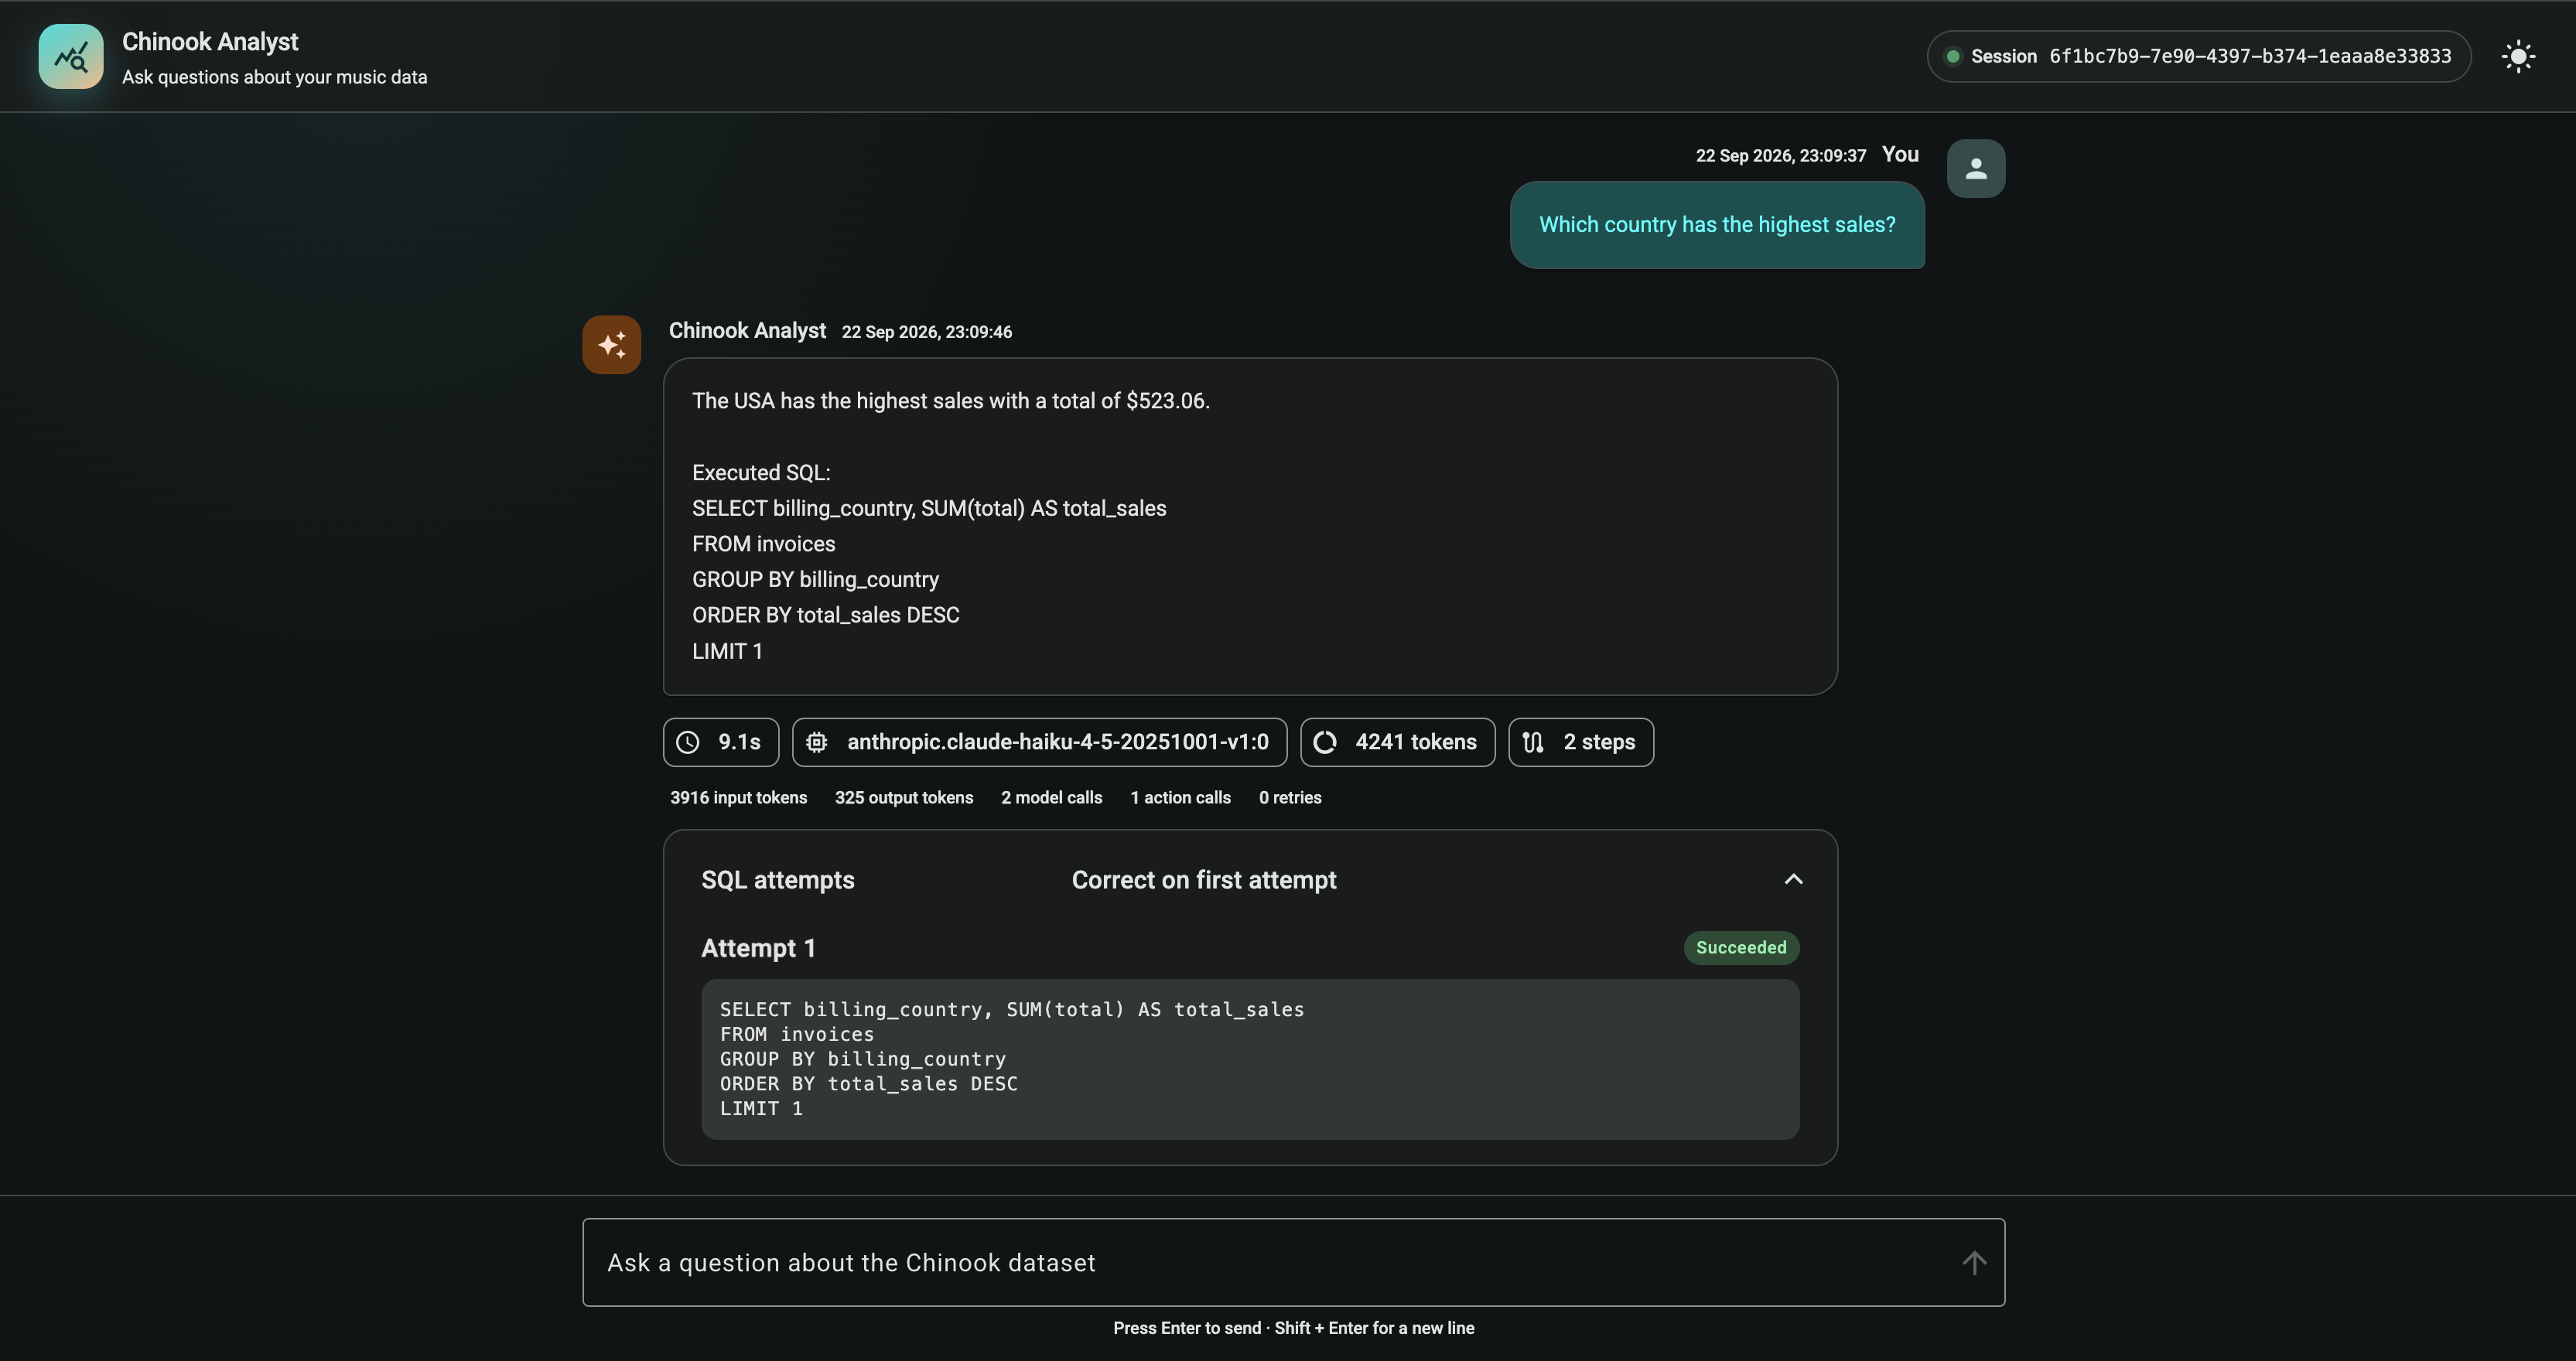
\includegraphics[width=13.5cm,trim=410bp 122.5bp 360bp 82.5bp,clip]
    {../../assets/chat-interface.png}};
% Leaders cross only unused background and stop beside the relevant content.
\foreach \number/\height/\endpoint in {1/-0.94/9.12,2/-2.65/0.87,3/-4.18/0.87,4/-6.07/0.87,5/-8.0/0.87} {
  \draw[leader] (0.25,\height)--(\endpoint,\height);
  \node[badge] at (0.25,\height) {\number};
}
% An aligned serif key, with consistent row spacing and no boxes or list indent.
\foreach \number/\height in {1/-11.05,2/-11.8,3/-12.55,4/-13.3,5/-14.05}
  \node[anchor=base,inner sep=0pt] at (0.25,\height) {\number};
\node[keylabel] at (0.8,-11.05) {User request};
\node[keytext] at (4.1,-11.05) {The natural-language question.};
\node[keylabel] at (0.8,-11.8) {Agent response};
\node[keytext] at (4.1,-11.8) {The answer returned to the user.};
\node[keylabel] at (0.8,-12.55) {Reported SQL};
\node[keytext] at (4.1,-12.55) {The query included in the agent's response.};
\node[keylabel] at (0.8,-13.3) {Request metrics};
\node[keytext] at (4.1,-13.3) {Duration, model, token usage and call counts.};
\node[keylabel] at (0.8,-14.05) {SQL attempts};
\node[keytext] at (4.1,-14.05) {Recorded query and execution status.};
\end{tikzpicture}
\end{document}
